%% ---- fig:sopdoc -- anatomy of one SOP document (SOP_Legalisir_Ijazah_Dan_Transkrip.pdf)
\begin{figure}[!htbp]
\centering
\resizebox{\textwidth}{!}{%
\begin{tikzpicture}[
  doc/.style={draw, fill=white, font=\scriptsize, align=left, inner sep=1.6mm, rounded corners=1pt},
  fld/.style={draw=blue!70!black, fill=blue!6, rounded corners=2pt, font=\scriptsize, align=left, inner sep=1.2mm, text width=52mm},
  tag/.style={font=\tiny\itshape, text=gray!40!black, anchor=east},
  map/.style={-{Stealth[length=1.6mm]}, gray!60!black, thin}
]
% ---------- left: the PDF page ----------
\node[doc, text width=74mm] (title) at (0,0)
  {\textbf{Standar Operasional Prosedur (SOP) Legalisir Ijazah Dan Transkrip}};
\node[doc, text width=74mm, anchor=north] (purp) at ([yshift=-1.2mm]title.south)
  {Dokumen ini berisi langkah-langkah \dots\ dengan total maksimal waktu pemrosesan maksimal 3 (tiga) hari kerja.};
\node[doc, text width=74mm, anchor=north] (step) at ([yshift=-1.2mm]purp.south)
  {1.\ \underline{Alumni} menyerahkan foto copy ijazah/transkrip nilai/sertifikat akreditasi program studi beserta surat aslinya kepada petugas Subbag Akademik dan Kemahasiswaan.};
\node[doc, text width=74mm, anchor=north] (wkt) at ([yshift=-1.2mm]step.south) {Waktu: $\pm$5 menit};
\node[doc, text width=74mm, anchor=north] (dok) at ([yshift=-1.2mm]wkt.south) {Dokumen yang dibutuhkan: Berkas Pengajuan Legalisir};
\node[doc, text width=74mm, anchor=north] (out) at ([yshift=-1.2mm]dok.south) {Output: Berkas Pengajuan Legalisir};
\node[font=\scriptsize, anchor=north west, text=gray!50!black] (more) at ([yshift=-0.6mm]out.south west) {2.\ Petugas Subbag Akademik dan Kemahasiswaan memeriksa \dots\quad 3.\ \dots\quad 6.\ \dots};
\node[tag] at ([xshift=-1mm]title.west) {title};
\node[tag] at ([xshift=-1mm]purp.west) {purpose};
\node[tag] at ([xshift=-1mm]step.west) {numbered step};
\node[tag] at ([xshift=-1mm]wkt.west) {time};
\node[tag] at ([xshift=-1mm]dok.west) {documents};
\node[tag] at ([xshift=-1mm]out.west) {output};
\begin{scope}[on background layer]
\node[draw=gray!50, fill=gray!6, rounded corners=3pt, inner sep=2mm, fit=(title)(more)] (page) {};
\end{scope}
\node[font=\scriptsize\bfseries, anchor=south west] at (page.north west) {(a) Source SOP document (one page, PDF)};
% ---------- right: graph attributes ----------
\node[fld, anchor=north west] (r1) at (8.7,0 |- title.north) {\textbf{Root} $v_{\text{root}}$\\ title: Legalisir Ijazah Dan Transkrip\\ max.\ duration: 3 hari kerja};
\node[fld, anchor=west] (s1) at (8.7,0 |- step.west) {\textbf{Step} $v_1$\quad actor: Alumni\\ action: Menyerahkan foto copy ijazah \dots\\ evidence: verbatim sentence of step 1};
\node[fld, anchor=west] (s2) at (8.7,0 |- wkt.west) {duration: $\pm$5 menit};
\node[fld, anchor=west] (s3) at (8.7,0 |- dok.west) {inputs: [Berkas Pengajuan Legalisir]};
\node[fld, anchor=west] (s4) at (8.7,0 |- out.west) {output: Berkas Pengajuan Legalisir};
\node[draw=blue!70!black, fill=white, rounded corners=3.5mm, font=\scriptsize, inner xsep=2mm, minimum height=6mm, anchor=west] (act) at (8.7,0 |- more.west) {$v_{\text{actor}}$: Alumni \ $\xrightarrow{\ \texttt{PERFORMS}\ }$\ $v_1$};
\begin{scope}[on background layer]
\node[draw=gray!50, fill=gray!6, rounded corners=3pt, inner sep=2mm, fit=(r1)(act)] (gph) {};
\end{scope}
\node[font=\scriptsize\bfseries, anchor=south west] at (gph.north west) {(b) Curated workflow-graph attributes};
% ---------- mapping arrows ----------
\draw[map] (title.east) -- (r1.west |- title.east);
\draw[map] (purp.east) -- (r1.west |- purp.east);
\draw[map] (step.east) -- (s1.west);
\draw[map] (wkt.east) -- (s2.west);
\draw[map] (dok.east) -- (s3.west);
\draw[map] (out.east) -- (s4.west);
\end{tikzpicture}}
\caption{Anatomy of an FSM SOP document and its mapping to workflow-graph attributes, shown for step 1 of the legalisation SOP. The underlined grammatical subject becomes the performing actor, the optional \emph{Waktu}, \emph{Dokumen yang dibutuhkan}, and \emph{Output} lines become duration, input, and output attributes, and the step sentence is stored verbatim as evidence.}
\label{fig:sopdoc}
\end{figure}

%% ---- fig:actors -- organisational roles x SOPs (PERFORMS edges of the workflow graph)
\begin{figure}[!htbp]
\centering
\resizebox{\textwidth}{!}{%
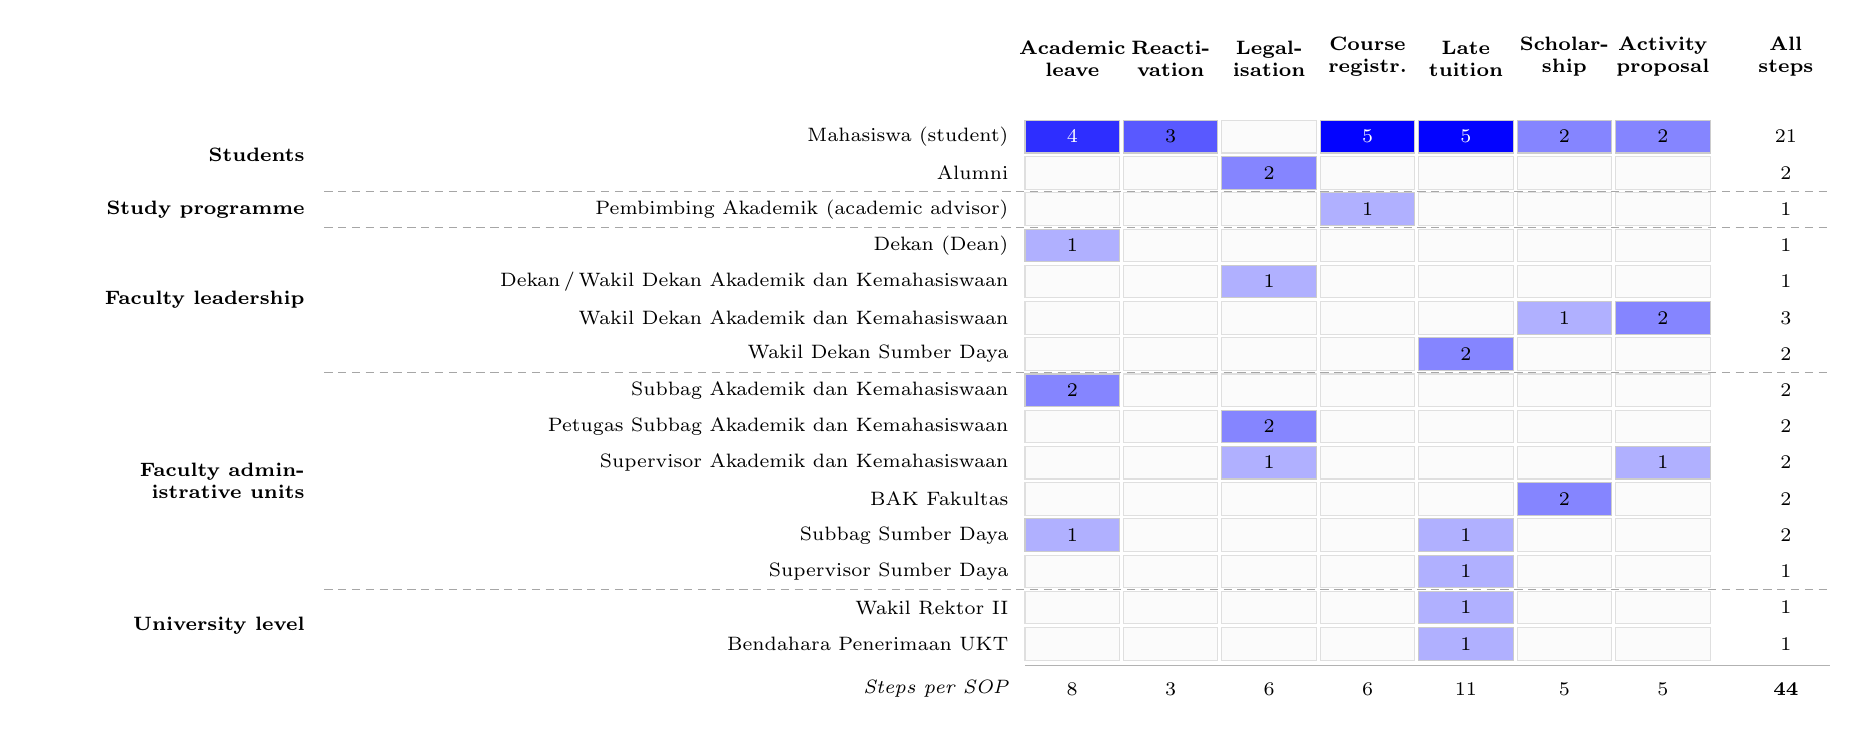
\begin{tikzpicture}[x=12.5mm, y=-4.6mm,
  rl/.style={anchor=east, font=\scriptsize},
  hd/.style={font=\scriptsize\bfseries, align=center, anchor=south},
  grp/.style={font=\scriptsize\bfseries, anchor=east, align=right, text width=34mm}
]
\def\cell#1#2#3{%
  \pgfmathsetmacro\shade{min(100,14+#3*17)}%
  \fill[blue!\shade!white, draw=gray!40] (#1-0.48,#2-0.45) rectangle (#1+0.48,#2+0.45);
  \node[font=\scriptsize, text=\ifnum#3>3 white\else black\fi] at (#1,#2) {#3};}
% column headers (SOPs)
\foreach \x/\t in {1/Academic\\leave, 2/Reacti-\\vation, 3/Legal-\\isation, 4/Course\\registr., 5/Late\\tuition, 6/Scholar-\\ship, 7/Activity\\proposal}
  \node[hd] at (\x,-0.4) {\t};
\node[hd] at (8.25,-0.4) {All\\steps};
% grid background
\foreach \y in {1,...,15} \foreach \x in {1,...,7}
  \draw[gray!25, fill=gray!3] (\x-0.48,\y-0.45) rectangle (\x+0.48,\y+0.45);
% rows: role labels
\foreach \y/\r in {
 1/Mahasiswa (student), 2/Alumni,
 3/Pembimbing Akademik (academic advisor),
 4/Dekan (Dean), 5/{Dekan\,/\,Wakil Dekan Akademik dan Kemahasiswaan}, 6/Wakil Dekan Akademik dan Kemahasiswaan, 7/Wakil Dekan Sumber Daya,
 8/Subbag Akademik dan Kemahasiswaan, 9/Petugas Subbag Akademik dan Kemahasiswaan, 10/Supervisor Akademik dan Kemahasiswaan, 11/BAK Fakultas, 12/Subbag Sumber Daya, 13/Supervisor Sumber Daya,
 14/Wakil Rektor II, 15/Bendahara Penerimaan UKT}
  \node[rl] at (0.45,\y) {\r};
% non-zero cells: column x, row y, steps performed
\cell{1}{1}{4}\cell{2}{1}{3}\cell{4}{1}{5}\cell{5}{1}{5}\cell{6}{1}{2}\cell{7}{1}{2}
\cell{3}{2}{2}
\cell{4}{3}{1}
\cell{1}{4}{1}
\cell{3}{5}{1}
\cell{6}{6}{1}\cell{7}{6}{2}
\cell{5}{7}{2}
\cell{1}{8}{2}
\cell{3}{9}{2}
\cell{3}{10}{1}\cell{7}{10}{1}
\cell{6}{11}{2}
\cell{1}{12}{1}\cell{5}{12}{1}
\cell{5}{13}{1}
\cell{5}{14}{1}
\cell{5}{15}{1}
% row totals
\foreach \y/\n in {1/21,2/2,3/1,4/1,5/1,6/3,7/2,8/2,9/2,10/2,11/2,12/2,13/1,14/1,15/1}
  \node[font=\scriptsize] at (8.25,\y) {\n};
% column totals
\draw[gray!60] (0.52,15.6) -- (8.7,15.6);
\node[rl, font=\scriptsize\itshape] at (0.45,16.25) {Steps per SOP};
\foreach \x/\n in {1/8,2/3,3/6,4/6,5/11,6/5,7/5} \node[font=\scriptsize] at (\x,16.25) {\n};
\node[font=\scriptsize\bfseries] at (8.25,16.25) {44};
% group separators and labels (administrative level)
\foreach \y in {2.5,3.5,7.5,13.5} \draw[gray!70, densely dashed] (-6.6,\y) -- (8.7,\y);
\node[grp] at (-6.7,1.5) {Students};
\node[grp] at (-6.7,3)   {Study programme};
\node[grp] at (-6.7,5.5) {Faculty leadership};
\node[grp] at (-6.7,10.5){Faculty administrative units};
\node[grp] at (-6.7,14.5){University level};
\end{tikzpicture}}
\caption{Organisational roles that perform SOP steps, grouped by administrative level, and the number of steps each performs per SOP (\texttt{PERFORMS} edges; darker cells denote more steps). Roles that only approve, sign, or receive copies within a step, such as the Head of Study Programme in the leave procedure, are recorded in action descriptions and not counted.}
\label{fig:actors}
\end{figure}
